% Created 2013-11-26 Tue 15:16
\documentclass{sigcomm-alternate}

\usepackage{amsmath}
\usepackage{booktabs}
\usepackage{algorithm}
\usepackage{algorithmic}
\usepackage{color}
\usepackage{graphicx}
\usepackage{listings}
\usepackage{subcaption}
\captionsetup{compatibility=false}
\usepackage{hyperref}
\usepackage{adjustbox}
\usepackage{tikz}
\usepackage{gnuplot-lua-tikz}
\usepackage{adjustbox}
\usepackage{fp}

\newcommand{\FIXME}[1]{{\color{red}\{FIXME #1\}}}

\lstset{language=C}
\definecolor{dkgreen}{rgb}{0,0.5,0}
\definecolor{dkred}{rgb}{0.5,0,0}
\definecolor{gray}{rgb}{0.5,0.5,0.5}
\lstset{basicstyle=\ttfamily\bfseries\footnotesize,
  morekeywords={virtualinvoke,fucompp,fnstsw,fldl,fstpl,movl},
  keywordstyle=\color{blue},
  ndkeywordstyle=\color{red},
  commentstyle=\color{dkred},
  stringstyle=\color{dkgreen},
  numbers=left,
  numberstyle=\ttfamily\footnotesize\color{gray},
  stepnumber=1,
  numbersep=10pt,
  backgroundcolor=\color{white},
  tabsize=4,
  showspaces=false,
  showstringspaces=false,
  xleftmargin=.23in
}
\date{\today}
\title{Automated Repair of Exploits in NETGEAR Router Binary}
\hypersetup{
  pdfkeywords={},
  pdfsubject={},
  pdfcreator={Emacs 24.3.1 (Org mode 8.2.3c)}}
\begin{document}

\maketitle
\usetikzlibrary{arrows,decorations,decorations.pathreplacing,shapes}

\begin{abstract}
Upon discovering a software exploit security researchers must decide
either to publish the exploit informing users and potential attackers,
or to privately inform the software vendor leaving users in the dark
and risking delay by the vendor.  We propose an alternative in which
researchers use the newly discovered exploits to drive an automated
repair technique capable of patching exploits with no access to source
code or special information from the software vendor.

We adapt existing evolutionary automated software repair techniques to
the special requirements of exploit repair.  We adapt the technique to
work on stripped MIPS ELF files, we remove the requirements for fault
localization information and we adapt the algorithm to work without
any pre-existing regression test suite.  We find that even without any
regression test suite 80\% of repairs of our example exploit retain
program functionality.

We demonstrate this approach by patching recently discovered exploits
in version 4 of NETGEAR's WNDR3700 wireless router \emph{before} NETGEAR
publicly addressed the exploits---to the author's knowledge NETGEAR
has not patched these exploits at the time of submission.  We discuss
the feasibility and utility of this technique for the security
community.
\end{abstract}

\section{Introduction}
\label{sec-1}
Security exploits pose significant monetary and social risks.  By
Symantec's count 5,291 vulnerabilities were reported in 2012
\cite{symantec2013threat}.

Upon discovering new exploits researchers are faced with a decision
between publicly announcing the exploit in a policy known as "full
disclosure" or privately informing the vendor of the exploit and
trusting the vendor to address the problem.  Although "full
disclosure" may increase attacks in the short term (In 2002, special
advisor for cyberspace security to then President Bush, Richard Clarke
said "It is irresponsible and\ldots{} extremely damaging to release
information before the patch is out") there are risks associated with
informing vendors as well (e.g., Oracle reportedly waited months after
researchers privately reported a bug in Java while thousands of users
were attacked before releasing a fix \cite{greenberg2012oracle}).

We propose a new option for security researchers in which reproducible
exploits are used to drive an automatic repair technique.  Such
patches may be either published with the exploit (it has been shown
that reporting an exploit with a patch in hand reduces the total
number of attacks \cite{arora2006does}), or sent privately to the
software vendor where they may speed the development of a patch
\cite{weimer06}.

In recent years automated methods of program repair have been shown
capable of repairing defects in real software \cite{forrest2009genetic,zeller2010,nguyen2013semfix,perkins2009automatically}.
Methods of evolutionary program repair have been developed which are
capable of repairing defects directly in x86 or ARM ELF files and
which require no access to program source code
\cite{schulte2013embedded}.  We adapt evolutionary program repair
techniques to the unique needs of security researchers who have no
access to either source code or to a regression test suite, and who
are generating repairs without any special information or cooperation
from the software vendor.  Although evolutionary program repair
techniques typically require access to a regression test suite, we
explore the feasibility of performing repair without any such test
suite and find that for our example exploit regression test suites are
most often not necessary.

We demonstrate the feasibility of this technique by patching security
vulnerabilities in the widely popular NETGEAR WNDR3700 wireless router
before NETGEAR publicly addressed the exploits.

In the remainder of this paper we; review two recent exploits to the
NETGEAR WNDR3700 (Section \ref{sec-2}), we demonstrate the feasibility
of running the NETGEAR firmware in a VM sandbox (Section \ref{sec-3-1}),
we review our novel techniques of automated program repair (Sections
\ref{sec-3-2} and \ref{sec-3-3}), and we evaluate the effectiveness of this
technique and the quality of the repairs it generates (Section
\ref{sec-4}).

The novel contributions of this short paper are;
\begin{enumerate}
\item an application of automated repair to stripped MIPS ELF files
recovered from router firmware
\item a modified version of evolutionary program repair which removes the
requirements for fault localization information, and for a
regression test suite
\item an application of automated repair to a real-world un-patched
security exploit resulting in
\item the first demonstration of multiple iterative repairs in a single
evolutionary run.
\end{enumerate}

In the pursuit of \emph{Reproducible Research} \cite{buckheit1995wavelab,mesirov2010accessible} and to encourage researchers to patch
future discovered exploits, we've released a companion version control
repository \footnote{\url{https://github.com/eschulte/netgear-repair}}.  This repository contains the instructions, source
code, and tooling needed to extract, execute and repair the binary
NETGEAR router image vulnerabilities.  All software needed to perform
repair work is freely available under open source licensing.
Additionally, the analysis performed in this document and all
supporting figures may be automatically regenerated from new
experimental data using the Org-mode reproducible research framework
\cite{schulte2012reproducible-research}.

We hope the ability to automatically patch vulnerable closed source
applications without dependence upon the software vendor encourages
users to patch vulnerable systems and researchers to release patches
with exploit announcements.
\section{Description of Exploits}
\label{sec-2}
In this work we repair a pair of exploits in version 4 of the popular
NETGEAR WNDR3700 wireless router.  The "shodan" \footnote{\url{http://www.shodanhq.com/search?q=wndr3700v4+http}} device search
engine returns hundreds of vulnerable publicly accessible WNDR3700
routers at the time of submission \cite{shodan}.  Both exploits exist in
the router's web server in a binary executable named \texttt{net-cgi}, and
both are related to how \texttt{net-cgi} handles authentication \cite{zcutlip}.

\begin{enumerate}
\item Any URI starting with the string "BRS" bypasses authentication.

\item Any URI including the string "unauth.cgi" or
"securityquestions.cgi" bypass authentication even pages of the
form "\url{http://router/page.html?foo=unauth.cgi}".
\end{enumerate}

Many administrative pages start with the "BRS" string, providing
attackers with access to personal information such as user's
passwords, and by accessing the page
"\url{http://router/BRS_02_genieHelp.html}" attackers can completely disable
authentication in a manner which is permanent across reboots.
\section{Repair Technique}
\label{sec-3}
To repair the \texttt{net-cgi} executable we must extract it and the router
file system from the firmware image distributed by NETGEAR.  Using the
extracted filesystem and executable we construct a test harness used
exercise the exploits in \texttt{net-cgi}.  This test harness is used by the
repair algorithm to evaluate candidate repairs and to identify when
repairs to the exploits have been found.

\subsection{Router Firmware Extraction and Virtualization}
\label{sec-3-1}
NETGEAR distributes firmware holding a full system image for the
WNDR3700 router which include the router file system holding the
vulnerable \texttt{net-cgi} executable.  Extraction of the file system may be
accomplished using \texttt{binwalk} \footnote{\url{http://binwalk.org}}, a firmware extraction tool which
scans the binary data in the firmware file searching for signatures
identifying the types of embedded data sections.  The \texttt{binwalk} tool
includes rules for identifying and extracting common embedded data
types, including a squashfs \cite{lougher2006squashfs} section which in
this case holds the router's file system.

The router runs on a big-endian MIPS architecture.  Using the QEMU
\cite{bellard2005qemu} system emulator to emulate this architecture a
Debian Linux operating system is run in emulation.  The extracted
router file system is copied into the emulated MIPS Linux system.  A
number of special directories (e.g., \texttt{/proc/}, \texttt{/dev/} etc\ldots{}) are
mounted inside the extracted file system and bound to the
corresponding directories on the virtual machine.  At this point
commands may be executed in an environment which closely approximates
the execution environment of the NETGEAR router using the \texttt{chroot}
command to confine executable access to within the extracted NETGEAR
file system.

With this accomplished (and with other minor adjustments described in
full in the reproduction information \footnote{\url{http://eschulte.github.io/netgear-repair/INSTRUCTIONS.html}}) is it possible to run
NETGEAR router in virtualization.  In particular the web interface of
the router may be accessed either using an external web browser or the
\texttt{net-cgi} executable may be called directly from the command line
using a Bash shell script \footnote{\url{https://github.com/eschulte/netgear-repair/blob/master/bin/test-cgi}}.
\subsection{Mutation of stripped MIPS ELF Files}
\label{sec-3-2}
The repair of ELF format files is an extension of the evolutionary
computation (EC) repair technique introduced in
\cite{schulte2013embedded}.  Mutation operations are used to modify the
execution behavior of the ELF file.  In this case the \texttt{net-cgi} file
is stripped a minimal ELF file which does not include much of the
information assumed to exist by the previous repair technique.

ELF (Executable and Linking Format) \cite{tis1995tool} files may either
be executed directly or may be linked with other object files to form
an executable or library.  The ELF file contains a number of headers
and tables containing administrative data, and sections holding
program code and data.  The three main administrative elements of an
ELF file are the ELF Header, the section table and the program table
(see Figure \ref{elf}).  The ELF Header points to the section table and the
program table, the section table holds information on the layout of
sections in the ELF file on disk, and the program table holds
information on how to copy section from disk into memory for program
execution.

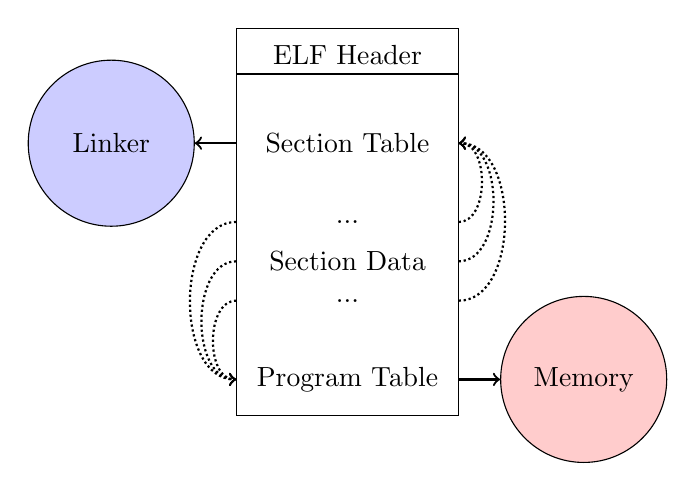
\begin{tikzpicture}
\label{elf}
  % ELF File
  \node[draw, rectangle, minimum height=14em, minimum width=8em] (whole) at (0,0) {};
  \node[minimum width=8em] (header) at (0,2.125) {ELF Header};
  \draw[thick] (header.south west) -- (header.south east);
  \node[minimum width=8em] (st) at (0,1) {Section Table};
  \node[minimum width=8em] (body1) at (0,-0) {...};
  \node[minimum width=8em] (body2) at (0,-0.5) {Section Data};
  \node[minimum width=8em] (body3) at (0,-1) {...};
  \node[minimum width=8em] (pt) at (0,-2) {Program Table};
  % External Users
  \node[draw, circle, fill=blue!20, minimum width=6em] (linker) at (-3,1) {Linker};
  \node[draw, circle, fill=red!20, minimum width=6em]  (memory) at (3,-2) {Memory};
  % Arrows to Users
  \draw[->,thick] (st.west) to (linker.east);
  \draw[->,thick] (pt.east) to (memory.west);
  % Section Table Arrows
  \draw[->,thick,densely dotted,bend right=90] (body1.east) to (st.east);
  \draw[->,thick,densely dotted,bend right=90] (body2.east) to (st.east);
  \draw[->,thick,densely dotted,bend right=90] (body3.east) to (st.east);
  % Program Table Arrows
  \draw[->,thick,densely dotted,bend right=90] (body1.west) to (pt.west);
  \draw[->,thick,densely dotted,bend right=90] (body2.west) to (pt.west);
  \draw[->,thick,densely dotted,bend right=90] (body3.west) to (pt.west);
\end{tikzpicture}

While the majority of ELF files include all three of these elements,
only the ELF Header is guaranteed to exist in all cases.  In
executable ELF files the program table is required, and in linkable
files the section table is required.

The previous ELF repair tool required a section table and a section
name string table, which were used to find the \texttt{.text} section of the
ELF file where program code is normally stored.  The data in the
\texttt{.text} section was then coerced into a "genome" a linear array of
assembly instructions which was modified by the mutation operations.
Our extension of this technique does not require a section table,
instead we build the genome by concatenating the data of every section
in the program table which has a "loadable" type.  These are the
sections whose data are loaded into memory during program execution.

Mutation operations must change program data without corrupting the
structure of the file or breaking the many addresses hard coded into
the program data itself (in general it is impossible to distinguish
between an integer literal and an address in program data).  For this
reason the mutation operations are designed to preserve the absolute
size and the offsets within of the ELF program data.  This is made
easier by the fact that MIPS is a RISC (Reduced Instruction Set
Computing) architecture in which every argumented assembly instruction
is 1 word long \cite{hennessy1982mips}.  The mutation and crossover
operations used to modify ELF files are shown in Figure \ref{mutation-ops}.

\tikzstyle{asmrow} = [rectangle, draw, minimum width=2em, minimum height=1em]
\begin{tikzpicture}
  % Mutation
  \foreach \x in {-3.5,-2.5,-0.5,0.5,2.5,3.5}{
    \foreach \y in {-0.8,-0.4,0,0.4,0.8}{
      \node[asmrow,fill=green!40] at (\x,\y) {};
    }
  }
  % Replace
  \node at (-3,1.25) {Replace};
  \node[asmrow,fill=yellow!20] (c-from) at (-3.5,0.4) {};
  \node[asmrow,fill=blue!60] at (-3.5,-0.4) {};
  % replace-after
  \node[asmrow,fill=yellow!20] at (-2.5,0.4) {};
  \node[asmrow,fill=yellow!20] (c-to) at (-2.5,-0.4) {};
  \node[asmrow,fill=green!40]  at (-2.5,-0.8) {};
  % Delete
  \node at (0,1.25) {Delete};
  \node[asmrow,fill=red!40] (d-from) at (-0.5,0) {};
  % delete-after
  \node[asmrow,fill=white] (d-to) at (0.5,0) {\scriptsize{0x0}};
  % Swap
  \node at (3,1.25) {Swap};
  \node[asmrow,fill=yellow!20] (s1-from) at (2.5,0.4) {};
  \node[asmrow,fill=blue!60] (s2-from) at (2.5,-0.4) {};
  % swap-after
  \node[asmrow,fill=blue!60] (s2-to) at (3.5,0.4) {};
  \node[asmrow,fill=yellow!20] (s1-to) at (3.5,-0.4) {};
  % arrows
  \draw[->,thick] (c-from.east) to (c-to.west);
  \draw[->,thick] (d-from.east) to (d-to.west);
  \draw[->,thick] (s1-from.east) to (s1-to.west);
  \draw[->,thick] (s2-from.east) to (s2-to.west);
  % Crossover
  \node at (0,-1.7) {One Point Crossover};
  \foreach \x in {-1.5,1.5}{
    \foreach \y in {-3.8,-3.4,-3,-2.6,-2.2}{
      \node[asmrow,fill=green!40] at (\x,\y) {};
    }
  }
  \foreach \x in {-0.5}{
    \foreach \y in {-3.8,-3.4,-3,-2.6,-2.2}{
      \node[asmrow,fill=blue!60] at (\x,\y) {};
    }
  }
  \draw[->,thick] (-2,-3.2) to (2,-3.2);
  \node[asmrow,fill=blue!60] at (1.5,-3.4) {};
  \node[asmrow,fill=blue!60] at (1.5,-3.8) {};
\end{tikzpicture}
\subsection{Lazy on demand Regression Testing}
\label{sec-3-3}
We present a novel evolutionary program repair algorithm which does
not require a pre-existing regression test suite.  We adopt the repair
algorithm from \cite{forrest2009genetic} but instead of assuming that a
regression test suite exists at the beginning of the algorithm, we
only assume that a single test case exists exercising an exploit.
High level pseudocode for the repair algorithm is show in Listing
\ref{lazy-algorithm}.

We then embark upon an interactive repair process in which the
algorithm fixes every available test (starting with only the exploit),
the user then determines the suitability of the evolved repair either
accepting the repair and terminating the algorithm, or rejecting the
repair and supplying a regression test which the repair fails.  If the
later, then the new test is incorporated into the test suite, and the
repair process continues.  In Section \ref{sec-4} we find that 80\% of our
attempts to repair the NETGEAR WNDR3700 exploits did not require any
regression tests be written.

\begin{figure}[H]
\begin{verbatim}
 1  # Input: Vulnerable Program, original: ELF
 2  # Input: Exploit Test, exploit: ELF -> Fitness
 3  # Input: Interactive Check, good-enough: ELF -> [ELF -> Fitness]
 4  # Output: Patched version of Program
 5  new <- null
 6  fitness <- null
 7  suite <- [exploit]
 8  do
 9    new <- minimize(evolutionary_subroutine(original, suite))
10    # User evaluates suitability of candidate repair
11    new-regression-tests <- good-enough(new)
12    suite <- suite ++ new-regression-tests
13  until length(new-regression-tests) == 0
14  return new
\end{verbatim}\caption{\label{lazy-algorithm}High-level Pseudocode for interactive lazy-regression-testing repair algorithm.}

\end{figure}

The \texttt{evolutionary\_subroutine} in Listing \ref{lazy-algorithm} has the same
high level organization as the evolutionary repair algorithm presented
in \cite{forrest2009genetic}, but it uses a \emph{steady state} evolutionary
computational algorithm \cite{Luke2013Metaheuristics} for reduced memory
usage and ease of parallelization of fitness evaluation.  High level
pseudocode for the \texttt{evolutionary\_subroutine} is shown in Listing
\ref{evolutionary-subroutine}.

\begin{figure}[H]
\begin{verbatim}
 1  # Input: Vulnerable Program, original: ELF
 2  # Input: Test suite, suite: [ELF -> Fitness]
 3  # Parameters: max-population-size, tournament-size, cross-rate
 4  # Output: Patched version of Program
 5  let fitness <- evaluate(original, suite)
 6  let pop <- max-pop-size copies of <original, fitness>
 7  do in every thread
 8    let p <- null
 9    if random() < cross-rate then
10      p <- crossover(tournament(pop,tournament-size,+),
11                     tournament(pop,tournament-size,+))
12    else
13      p <- tournament(pop,tournament-size,+)
14    endfi
15    p <- mutate(p)
16    fitness <- evaluate(suite, p)
17    incorporate(pop, <p, fitness>)
18    if length(pop) > max-population-size then
19      evict(pop, tournament(pop,tournament-size,-))
20    endif
21  until fitness > length(suite)
22  return p
\end{verbatim}\caption{\label{evolutionary-subroutine}High-level Pseudocode for the steady state parallel evolutionary repair subroutine.}

\end{figure}

A careful reader will notice that every time the user rejects the
solution returned by \texttt{evolutionary\_subroutine} the evolved and
minimized solution is discarded and a new population is generated by
again copying the original by the \texttt{evolutionary\_subroutine}.  Unlike
in most applications of EC, but as in nature, EC of extant programs
always starts from a point in the fitness landscape which is very
nearly optimal.  This is because the original program is not a random
guess, but is a highly engineered solution to the program fitness
landscape.  This algorithmic choice acknowledges the fitness of the
original program, and for this reason gives it primacy over the
evolved solutions of previous iterations (which may well have evolved
into fitness valleys as in run 8 Table \ref{minimized-stats}).
\section{Repair Demonstration}
\label{sec-4}
\subsection{Methodology}
\label{sec-4-1}
We demonstrate our technique by patching two NETGEAR WNDR3700
exploits.  All repairs were performed on a server-class machine with
32 physical Intel Xeon 2.60GHz cores, Hyper-Threading and 120 GB of
Memory.  To perform fitness evaluations we use 32 QEMU virtual
machines, each running Debian Linux with the NETGEAR router firmware
environment available inside of a \texttt{chroot}.

The test framework includes both a host and a guest test script.  The
host script copies a variant of the \texttt{net-cgi} executable to the guest
VM, and invokes the guest test script which runs \texttt{net-cgi} on the
command line and reports the result of "PASS" "FAIL" or "ERROR" of
each test back to the host test script, which uses these values to
calculate a scalar fitness for the variant.

We report the results of 10 repair attempts, each following the high
level algorithm shown in Listing \ref{lazy-algorithm} and using the
following EC parameters.

\subsubsection{Repair Parameters}
\label{sec-4-1-1}
Repair was run using the parameters shown in Table \ref{parameters}.  The
maximum population size was 512 individuals, selection is performed
using a tournament size of 2.  When the population overflows the
maximum population size, an individual is selected for eviction using
a negative tournament of size 2.  Newly selected individuals are
crossed over $\frac{2}{3}$'s of the time.

\begin{table}[htb]
\centering
\begin{tabular}{lr}
parameter & value\\
\hline
max-population-size & 512\\
tournament-size & 2\\
cross-rate & $\frac{2}{3}$\\
\end{tabular}\caption{\label{parameters}The parameters used to evolve repairs to the NETGEAR WNDR3700 exploits.}

\end{table}

These parameters differ significantly from those used in previous EC
repair algorithms \cite{forrest2009genetic,legoues2011systematicstudy,le2012representations} in that we
use larger populations (of 512 instead of 40 individuals), running for
many more fitness evaluations ($\leq$100,000 instead of $\leq$400).  The
parameters used in this paper are more inline with traditional EC
parameters given the size of the software genome, and allow our
technique to overcome the lack of any fault localization information.

The increased memory required by the larger population size is offset
by the use of a steady state EC algorithm, and the increased
computational demand of the greater number of fitness evaluations is
offset by parallelization of fitness evaluation.
\subsubsection{Repair Runtime}
\label{sec-4-1-2}
The repair algorithm itself uses 32 threads for parallel fitness
evaluation.  Each thread is paired with a single QEMU VM on which it
tests fitness.  When any thread finds a repair the inner repair loop
(\texttt{evolutionary\_subroutine}) of the algorithm terminates globally and
the candidate repair is presented to the user (line 11 of Listing
\ref{lazy-algorithm}).

The time taken to perform a fitness evaluation varies with the size of
the regression suite.  Table \ref{test-speed} shows the average number of
fitness evaluations performed in our setup per minute over a variety
of regression test sizes.

\begin{table}[htb]
\centering
\begin{tabular}{lrrrr}
suite size & 0 & 1 & 5 & 10\\
\hline
evals per minute w/32 cores & TODO &  &  & \\
\end{tabular}\caption{\label{test-speed}Using 32 virtual machines to evaluate fitness in parallel we are able to perform the following number of fitness evaluation per minute as a function of regression suite size.}

\end{table}
\subsection{Analysis of Repairs}
\label{sec-4-2}
\subsubsection{Iterative Repair}
\label{sec-4-2-1}
The repairs required two distinct fixes to two different exploits in a
single long evolutionary run.  This is an instance of "iterative
repair" which has not previously been observed in the repair of
real-world extant software.

\url{fitness-improvement.tex}
\subsubsection{Minimization Impact}
\label{sec-4-2-2}
In many cases the initial evolved repair broke untested behavior.  For
example evolved repairs sometimes worked when \texttt{net-cgi} was called
directly on the command line but not through the embedded
µHTTPd \footnote{\url{http://wiki.openwrt.org/doc/uci/uhttpd}} webserver, or the evolved file failed to serve pages not
used in the exploit test.  As shown in Table \ref{minimized-stats}, in most
cases the minimized version of the evolved executable fixed all of the
regressions found in the evolved repair.  The functionality numbers in
Table \ref{minimized-stats} were generated using a hand-written regression
test suite.

\begin{table}[htb]
\centering
\begin{tabular}{rrrrrr}
Run Id & Fit Evals & Full Diff & Min Diff & Full Fit & Min Fit\\
\hline
0 & 90405 & 500 & 2 & 8 & 22\\
1 & 17231 & 134 & 3 & 22 & 22\\
2 & 26879 & 205 & 2 & 21 & 22\\
3 & 23764 & 199 & 2 & 19 & 22\\
4 & 47906 & 319 & 2 & 6 & 6\\
5 & 13102 & 95 & 2 & 16 & 22\\
6 & 76960 & 556 & 3 & 17 & 22\\
7 & 11831 & 79 & 3 & 20 & 22\\
8 & 2846 & 10 & 1 & 14 & 14\\
9 & 25600 & 182 & 2 & 21 & 22\\
\hline
mean & 33652.4 & 227.9 & 2.2 & 16.4 & 19.6\\
\end{tabular}\caption{\label{minimized-stats}Difference and functionality of evolved repair before and after minimization.  In these columns "Full" refers to evolved solutions before minimization and "Min" refers to post-minimization solutions.  Columns labeled "Diff" report the number of unified diff windows against the original program data. The columns labeled "Fit" report the fitness measured with a full regression test suite including the exploit tests with a maximum fitness of 22.}

\end{table}
\subsubsection{Repair Size}
\label{sec-4-2-3}
As shown in Table \ref{minimized-stats}, the initial evolved repair differed
from the original at >200 locations on average in the ELF program
data, while the minimized repairs differed at only 1-3 locations on
average.  This great discrepancy is due to the accumulation of edits
in non-tested portions of the program data.  Since these portions of
the genome were not tested there was no evolutionary pressure to purge
harmful edits.  The elimination of these accumulated edits is the main
purpose of minimization, and is the reason for the consistent increase
in regression test behavior found in the minimized repairs.
\section{Related Work}
\label{sec-5}
\subsection{Security}
\label{sec-5-1}
There has been a significant effort to understand the impacts of
disclosure of discovered exploits.  Researchers typically must decide
between public disclosure (termed "full disclosure") or private
disclosure to the vendor of the vulnerable software.  The former
increases the number of attacks in the short term \cite{arora2006does},
while the later risks the vendor ignoring the exploit extending the
life of the exploit.

Even major software vendors commonly delay releasing patches to
security exploits.  Microsoft waits until the second Tuesday of every
month (known as "Patch Tuesday") to release security patches
\cite{lemos2003microsoft}, leading malicious users to release new
exploits on the second Wednesday of every month (known as "Exploit
Wednesday") to maximize the time before a patch is released.

In a study of high and medium risk vulnerabilities in Microsoft and
Apple products between 2002 and 2008, \textasciitilde{}10\% of vulnerabilities were
found not to be patched within 150 days of disclosure, and on any
given date $\sim$10 vulnerabilities and >20 vulnerabilities were public and
un-patched for Microsoft and Apple respectively \cite{frei20080}.

The question of when to report an exploit has been studied is not
easily decidable in all cases \cite{arora2008optimal}.
\subsection{EC}
\label{sec-5-2}
TODO: EC background
\subsection{Automated Program Repair}
\label{sec-5-3}
TODO
\begin{itemize}
\item genprog
\item clearview
\item semfix
\end{itemize}
\section{Discussion}
\label{sec-6}
This technique demonstrates the ability of end users to fix software
exploits in closed source software without any special information or
aid from the software vendor.

\subsection{Threats to Validity}
\label{sec-6-1}
This initial work is based upon a single exploit repair so it is
possible that the results indicating the effectiveness of repair
without any regression test suite will not generalize.  However, the
authors do not believe that these results are based on any property
unique to the NETGEAR exploits, rather we believe that the ability of
the evolutionary repair algorithm to find functional repairs without
the use of any regression test suite is due to both the beneficial
impact of minimization, and to the natural mutational robustness of
software (cf. \cite{schulte2013software}).  Specifically in
\cite{schulte2013software} Schulte et al. find that the functionality of
software mutants differs by only \textasciitilde{}60\% between software tested with a
null regression test suites and software tested with the best
obtainable quality regression test suites.
\subsection{Next Steps}
\label{sec-6-2}
\begin{itemize}
\item operation directly on a binary image
\begin{itemize}
\item would require better virtualization
\item would require better fault localization
\end{itemize}
\item proactive hardening
\begin{itemize}
\item shutting off (read:breaking) insecure functionality such as
password reset
\item combination with a fuzz tester in a closed exploit/repair loop
\end{itemize}
\item distributed diversity
\begin{itemize}
\item self certifying patches
\end{itemize}
\end{itemize}
\section{Acknowledgments}
\label{sec-7}
Foremost we'd like to thank Zachary Cutlip who analyzed and announced
the NETGEAR exploits, and who helped us to reproduce the exploits
locally.  Without his help this work would not have been possible.  We
would also like to thank Mark Harman for discussion of program repair
without a regression test suite, and Stephen Harding for initially
formulating the interactive lazy regression repair algorithm.

Also, GRANTS GRANTS GRANTS.

\bibliographystyle{plain}
\bibliography{netgear-repair}
% Emacs 24.3.1 (Org mode 8.2.3c)
\end{document}